% !TeX spellcheck = hu_HU
\documentclass[12pt,a4paper]{article}
\usepackage[utf8]{inputenc}
\usepackage{cmap}
\usepackage[T1]{fontenc}
\usepackage[magyar]{babel}
\usepackage{amsmath}
\usepackage{amsfonts}
\usepackage{amssymb}
\usepackage{graphicx}

\usepackage{struktex}
\usepackage{outlines}
\usepackage{hyperref}

\hyphenpenalty=10000

%TeXstudio doesn't like leadsto by default
\renewcommand{\leadsto}{\rightsquigarrow}

\begin{document}

\begin{center}
	\huge
	Algoritmusok és adatszerkezetek II\\
	\vspace{1mm}
	\LARGE
	Gráfok témakör jegyzete\\
	\vspace{5mm}
	\large
	Készült Ásványi Tibor előadásai és gyakorlatai alapján\\
	\vspace{5mm}
	Sárközi Gergő, 2021-22-1. félév\\
	Nincsen lektorálva!
\end{center}

\tableofcontents

\pagebreak

\section{Egyszerű gráfok és ábrázolásaik}

\subsection{Definíciók}

\subsubsection{Gráf}

\begin{outline}
	\1 $G=(V,E)$ rendezett pár
	\1 $V$ a csúcsok véges halmaza
		\2 $V=\{\}$ üres gráf
	\1 $E \subseteq V \times V \ \{(u,u) | u \in V\}$ az élek halmaza
		\2 hurokéleket explicit, párhuzamos éleket implicit kizártuk
		\2 tehát gráf = egyszerű gráf a továbbiakban
\end{outline}

\subsubsection{Irányítottság}

\begin{outline}
	\1 gráf irányítatlan, ha $(u,v) \in E \Leftrightarrow (v,u) \in E$
	\1 gráf irányított, ha nem következik az egyik a másikból
	\1 irányított $G=(V,E)$ gráf irányítatlan megfelelője:
		\2 $G'=(V,E')$ ahol $E'=\{(u,v) | (u,v) \in E \wedge (v,u) \in E\}$
\end{outline}

\subsubsection{Út}

\begin{outline}
	\1 út: $<u_0, u_1, u_2, ...,u_n>$ ($u_i \in V$ és $(u_{i-1},u_i) \in E$)
		\2 ekkor az út hossza $n$ (ami az élek száma is)
	\1 rész-út: logikusan
	\1 kör: kezdő és végpontja azonos, $n>0$ és minden éle különböző
		\2 nincs hurokél: $n \ge 2$
	\1 körmentes út: nem tartalmaz kört (nincs olyam részútja, ami kör)
	\1 körmentes gráf: csak körmentes utak vannak benne
\end{outline}

\pagebreak

\subsubsection{DAG (irányított, körmentes gráf)}

\begin{outline}
	\1 Directed Acyclic Graph
\end{outline}

\subsubsection{Összefüggőség}

\begin{outline}
	\1 G irányítatlan gráf összefüggő, ha mindegyik két csúcsa között van út
	\1 G irányított gráf összefüggő, ha az irányítatlan megfelelője összefüggő
	\1 generátor csúcs: ha tetszőleges csúcs elérhető belőle (van út köztük)
		\2 csak irányított gráfoknál van értelme
		\2 van generátor csúcs $\implies$ összefüggő (fordítva nem)
\end{outline}

\subsubsection{Fa}

\begin{outline}
	\1 szabad fa, irányítatlan fa: irányítatlan, körmentes, összefüggő gráf
	\1 gyökeres fa, irányított fa: irányított gráf aminek van generátor csúcsa
	és az irányítatlan megfelőle körmentes
		\2 ekkor a generátor csúcs a gyökér csúcs
	\1 nemüres fának pontosan eggyel kevesebb éle van, mint csúcsa
	\1 erdő: összefüggő komponensei fák (vagy egyetlen fából áll)
		\2 irányítatlan G gráf erdő $\Leftrightarrow$ G körmentes
		\2 irányított G gráf erdő $\Leftrightarrow$ G irányítatlan megfelelője körmentes
		és G mindegyik összefüggő komponensének van generátor csúcsa
\end{outline}

\subsubsection{Részgráf}

\begin{outline}
	\1 $G=(V,E)$ gráfnak részgráfja a $G'=(V',E')$ gráf, ha:
		\2 mindkét gráf irányított vagy mindkét gráf irányítatlan
		\2 $V' \subseteq V$ és $E' \subseteq E$
	\1 valódi részgráf: $G \ne G'$
	\1 diszjunkt részgráfok: nincs közös csúcsok (és ezáltal közös élük sem)
	\1 összefüggő komponens: olyan részgráf, aminek nincs összefüggő részgráfja
		\2 minden gráf vagy összefüggő, vagy felbontható diszjunkt összefüggő komponensekre
\end{outline}

\pagebreak

\subsection{Gráfábrázolás alapjai}

\begin{outline}
	\1 Legyen $V=\{v_1, v_2, ..., v_n\}$
	\1 Számok helyett gyakran használunk betűket (a=1, b=2, ...)
	\1 Legyen $n=|V|$ és $m=|E|$, ekkor $0\le m \le n*(n-1) \le n^2$
		\2 azaz $m \in O(n^2)$
		\2 ritka gráf: $m \in O(n)$
		\2 sűrű gráf: $m \in \Theta(n^2)$
\end{outline}

\subsection{Grafikus gráfábrázolás}

\begin{outline}
	\1 Csúcs: kör (bele írjuk a csúcs sorszámát)
	\1 Irányítatlan él: vonal
	\1 Irányított él: nyíl
\end{outline}

\subsection{Szöveges ábrázolás}

\begin{outline}
	\1 Irányítatlan gráf: $u - u_1 ; u_2 ; u_3 ; ...$
		\2 $u$ csúcsnak szomszédai a $u_1$, $u_2$, stb. csúcsok
		\2 nem kell oda-vissza feltünteni (tehát lehet mindent növekvő sorrendben leírni)
	\1 Irányított gráf: $u \to u_1 ; u_2 ; u_3 ; ...$
		\2 $u$ csúcsból vezet él a $u_1$, $u_2$, stb. csúcsokba
\end{outline}

\pagebreak

\subsection{Szomszédossági mátrix (adjacency matrix), avagy csúcsmátrixos ábrázolás}

\begin{outline}
	\1 $A/1 : bit[n,n]$ mátrix, ahol bit=\{0,1\} és $n=|V|$
		\2 $A[i,j] = 1 \Leftrightarrow (v_i,v_j) \in E$
		\2 $A[i,j] = 0 \Leftrightarrow (v_i,v_j) \notin E$
		\2 $i$ a sor, $j$ az oszlop: sorszámból vezet oszlopszámba él
	\1 főátlóban mindig 0-k vannak, mert csak egyszerű gráfokkal foglalkozunk
		\2 $A[i,i] = 0$
	\1 irányítatlan gráf: főátlóra szimmetrikus mátrix
		\2 $A[i,j] = A[j,i]$
		\2 emiatt $n^2$ helyett elég $n*(n-1)/2$ hosszú tömb a mátrix ábrázolására\\
		(általában az alsó háromszögmátrixot választjuk, főátló nélkül)
\end{outline}

\subsection{Szomszédossági listás (adjacency list) ábrázolás}

\begin{outline}
	\1 hasonlít a szöveges reprezentációhoz
	\1 az i. csúcs szomszédainak sorszámát a $A[i]$ S1L tartalmazza
		\2 valójában: $A/1 : Edge*[n]$, ahol $Edge$ tagjai: $v$, $next$
	\1 irányítatlan gráfok esetén minden él így kétszer van tárolva
	\1 tárigénye: $n$ db mutató, listáknak összesen $m$ vagy $2*m$ elem
		\2 azaz mindkét esetben $\Theta(n+m)$
		\2 ritka gráf: $\Theta(n)$ (mert $m \in O(n)$)
		\2 sűrű gráf: $\Theta(n^2)$ (mert $m \in O(n^2)$)
\end{outline}

\pagebreak

\section{Absztrakt halmaz, sorozat, gráf}

\subsection{Absztrakt halmaz}

\begin{outline}
	\1 $T$ típusú véges halmaz: $T\{\}$
	\1 $s : T\{\}$ egy üres halmaz, $s : T\{a,b,c\}$ egy 3 elemű halmaz
	\1 kiválasztás (tetszőleges elem eltávolítása): $u \;from\; S$
		\2 $S$ egy nemüres halmaz
		\2 $S$-ből eltávolítunk egy elemet és ezt $u$ értékül kapja
\end{outline}

\subsection{Absztrakt sorozat}

\begin{outline}
	\1 $T$ típusú véges sorozat: $T<>$
	\1 $s : T<>$ egy üres sorozat, $s : T<a,b,c>$ egy 3 elemű sorozat
	\1 1-től indexeljük őket
	\1 ha $u,v : T<>$ akkor $u+v$ a konkatenálás
\end{outline}

\subsection{Absztrakt gráf}

\begin{outline}
	\1 $\mathcal{V}$: vertex (csúcs) típus
		\2 tetszőlegesen sok, névvel jelölt, értékkel ellátott címkét tárol
		\2 legyen $v$ csúcs, $name$ a címke neve, ekkor $name(v)$ a címke értéke
	\1 $\mathcal{E}$: edge (él) típus, adattagjai: $u,v : \mathcal{V}$
	\1 $\mathcal{G}$: élsúlyozatlan absztrakt gráf
		\2 adattagok: $V:\mathcal{V}\{\}$ és $E:\mathcal{E}\{\}$
		\2 $V$ véges
		\2 $E \subseteq V \times V \setminus \{(u,u) | u \in V\}$
\end{outline}

\pagebreak

\section{Elemi gráfalgoritmusok}

\begin{outline}
	\1 gráfok nincsenek élsúlyozva
\end{outline}

\subsection{BFS (szélességi gráfkeresés)}

\begin{outline}
	\1 irányított és irányítatlan gráfokra is értelmezett
	\1 egy adott csúcsból ($s$) meghatározza az összes másik csúcsba vezető legrövidebb utat
	\1 használt címkék:
		\2 $d$: távolság a kezdő csúcstól
		\2 $\pi$: "szülő", azaz a kezdő csúcs felé levő úton az első csúcs
			\3 $\pi(s)=\emptyset$
		\2 ha $u$ egy el nem érhető csúcs: $pi(u)=\emptyset$ és $d(u)=\infty$
		\2 $color$: csak vizualizáció miatt
			\3 fehér: még nincs megtalálva
			\3 szürke: feldolgozásra vár
			\3 fekete: feldolgozva
	\1 indeterminisztikus esetekben a kisebb címkéjű csúcsot válasszuk
	\1 időkomplexitás
		\2 legyen $n=|G.V|$ és $m=|G.E|$
		\2 $MT(n,m) \in \Theta(n+m)$ (2. ciklus max m-szer iterál)
			\3 szomszédossági listás ábrázolás esetén: $\Theta(n^2)$
		\2 $mT(n,m) \in \Theta(n)$ (2. ciklus min egyszer iterál)
\end{outline}

\pagebreak

\begin{figure}[h!]
	\centering
	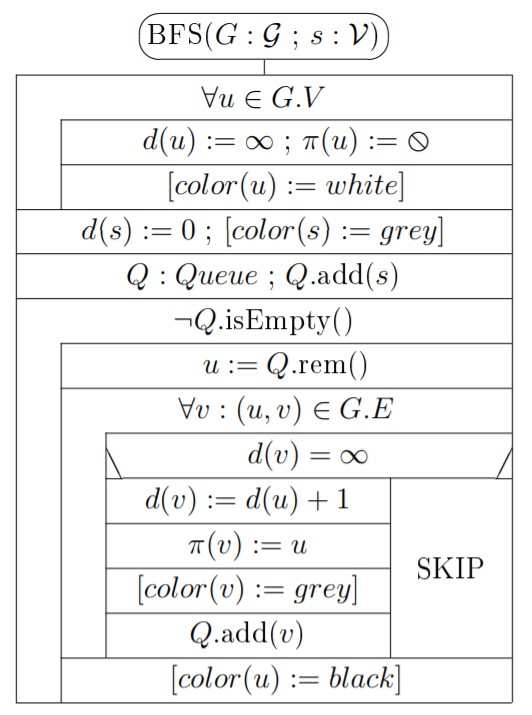
\includegraphics[width=0.5\linewidth]{bfs}
\end{figure}

\subsubsection{Szélességi fa (Breadth-first tree)}

\begin{outline}
	\1 ha $\pi(u)=v$-t úgy értelmezzük, hogy $v$ szüleje $u$-nak, akkor fát kapunk
	\1 más néven: legrövidebb utak fája
\end{outline}

\pagebreak

\subsection{DFS (Mélységi gráfkeresés)}

\begin{outline}
	\1 egyszerű, irányított gráfokra értelmezett
	\1 használt címkék:
		\2 d: elérési idő (discovery time)
		\2 f: befejezési idő (finishing time)
		\2 $\pi$: "szülő", azaz a kezdő csúcs felé levő úton az első csúcs
			\3 $\emptyset$, ha egy mélységi fa gyökere
		\2 color: (nem kihagyható)
			\3 fehér: érintetlen
			\3 szürke: belőle elérhető csúcsokat járunk be éppen
			\3 fekete: feldolgozva
	\1 DFSvisit mélységi fát számol ki, DFS pedig mélységi feszítő erdőt
	\1 time akkor lép, amikor elérünk vagy befejezünk egy csúcsot
		\2 az első time érték = 1
	\1 backEdge(u,v): tetszőleges eljárás, tegyük fel, hogy $\Theta(1)$
	\1 időkomplexitás:
		\2 legyen $n=|G.V|$ és $m=|G.E|$
		\2 DFSvisit n-szer hívódik, de a ciklusa ÖSSZESEN csak m-et iterál
		\2 $MT(n,m),mT(n,m) \in \Theta(n+m)$
\end{outline}

\begin{figure}[h!]
	\centering
	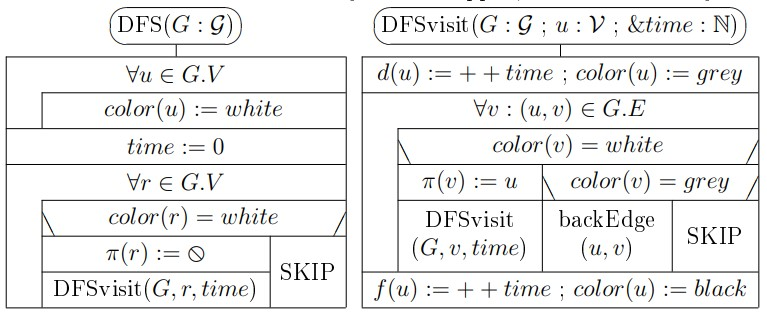
\includegraphics[width=0.85\linewidth]{dfs}
\end{figure}

\pagebreak

\subsubsection{Élek osztályozása}

\begin{outline}
	\1 (u,v) fa-él (tree edge): (u,v) valamelyik mélységi fa éle.\\
	(Ezen élek mentén járjuk be a gráfot.)
	\1 (u,v) vissza-él (back edge): v az u őse, de nem faél.
		\2 Ez azt jelenti, hogy irányított kört találtunk.
	\1 (u,v) előre-él (forward edge): v az u leszármazottja, de nem faél.
	\1 (u,v) kereszt-él (cross edge): u és v két olyan csúcs, amelyek vagy azonos mélységi fa két különböző ágán vannak, vagy két különböző mélységi fában vannak.
\end{outline}

\subsubsection{Élek felismerése}

Mélységi bejárás során az (u,v) él feldolgozásakor:\\
(Ha szöveges címkét rendelnénk a feldolgozás során, így tennénk.)

\begin{outline}
	\1 (u,v) fa-él: v csúcs még fehér
	\1 (u,v) vissza-él: v csúcs éppen szürke
	\1 (u,v) előre-él: v csúcs már fekete és $d(u) < d(v)$
	\1 (u,v) kereszt-él: v csúcs már fekete és $d(u) > d(v)$
\end{outline}

\subsubsection{Bejárás szemléltetése}

\begin{outline}
	\1 Élek: dupla a fa él, többi betűvel jelölve
	\1 csúcsnál x/y: d(u) / f(u)
\end{outline}

\begin{figure}[h!]
	\centering
	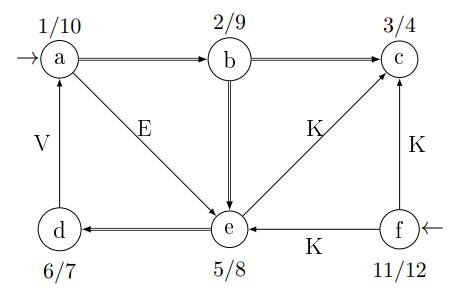
\includegraphics[width=0.5\linewidth]{dfs-példa}
\end{figure}

\pagebreak

\subsubsection{DAG tulajdonság eldöntése}

\begin{outline}
	\1 $G$ irányított gráf akkor Directed Acyclic Graph, ha nem tartalmaz irányított kört
	\1 DFS fog találni vissza-élt, ha van irányított kör a gráfban
		\2 viszont nem fog annyi vissza-élt találni, ahány irányított kör van:
		egy él lehet több kör része is
	\1 $(u,v)$ vissza-él $\implies$ $<u,v,...,\pi(\pi(u)),\pi(u),u>$ egy irányított kör
		\2 ezt a kört az algoritmus a fordított sorrendben találná meg
	\1 a backEdge eljárás hasznos eme infó lementése céljából
\end{outline}

\subsubsection{Topologikus rendezés}

\begin{outline}
	\1 Topologikus rendezés: gráf csúcsainak olyan sorba rendezése, hogy minden él egy későbbi csúcsba mutasson. (Pl. minden él balról jobbra.)
	\1 Irányított gráfnak lehet 0, 1 vagy több féle topologikus rendezése.
	\1 Irányított gráfnak pontosan akkor van topologikus rendezése, ha DAG.
	\1 Mélységi bejárás segítségével topologikus rendezés:
		\2 csúcsok $f(u)$ szerint csökkenő rendezése
		\2 vagy csúcsokat befejezésükkör rakjuk egy verembe
\end{outline}

\pagebreak

\section{Élsúlyozott gráfok és ábrázolásaik}

\subsection{Absztrakt ábrázolás}

\begin{outline}
	\1 $\mathcal{V}$: vertex (csúcs) típus, címkéket tárol, lásd normál gráf
	\1 $\mathcal{E}$: edge (él) típus, adattagjai: $u,v : \mathcal{V}$
	\1 $\mathcal{G}_w$: élsúlyozott absztrakt gráf
		\2 adattagok: $V:\mathcal{V}\{\}$, $E:\mathcal{E}\{\}$ és $w:E \to \mathbb{R}$
		\2 $V$ véges
		\2 $E \subseteq V \times V \setminus \{(u,u) | u \in V\}$
		\2 $w$ a súlyfüggvény
\end{outline}

\subsection{Emlékeztető}

\begin{outline}
	\1 $n=|V|$ és $m=|E|$
	\1 $0 \le m \le n*(n-1) \le n^2$
	\1 ritka gráf: $m \in O(n)$
	\1 sűrű gráf: $m \in \Theta(n^2)$
\end{outline}

\subsection{Grafikus ábrázolás}

\begin{outline}
	\1 Csúcs: kör (bele írjuk a csúcs sorszámát)
	\1 Irányítatlan él: vonal; irányított él: nyíl
	\1 Élek mellé odaírjuk a súlyukat
\end{outline}

\subsection{Szöveges ábrázolás}

\begin{outline}
	\1 Irányítatlan gráf: $v - v_1, w_1 ; v_2, w_2 ; ...$
		\2 $v$ csúcsnak szomszédai a $v_i$ csúcsok, az él súlya $w_i$
		\2 nem kell oda-vissza feltünteni (tehát lehet mindent növekvő sorrendben leírni)
	\1 Irányított gráf: $v \to v_1, w_1 ; v_2, w_2 ; ...$
		\2 $u$ csúcsból vezet él a $u_i$ csúcsokba, $w_i$ élsúllyal
\end{outline}

\pagebreak

\subsection{Szomszédossági mátrix, csúcsmátrix, adjacency matrix}

\begin{outline}
	\1 $A\rightarrow : \mathbb{R}_\infty[n,n]$ ahol $n=|V|$
		\2 $A[i,i] = 0$ (egyszerű gráf)
		\2 $A[i,j] = \infty \Leftrightarrow (v_i,v_j) \notin E$
		\2 $A[i,j] = w(v_i,v_j) \Leftrightarrow (v_i,v_j) \in E$
		\2 i a sor, j az oszlop: sorszámból vezet oszlopszámba él
	\1 Irányítatlan gráf: főátlóra szimmetrikus
	\1 Tárigény $\Theta(n^2)$ (ha egy $\mathbb{R}_\infty$ konstans hosszú)
\end{outline}

\subsection{Szomszédossági lista, adjacency list}

\begin{outline}
	\1 Hasonlít a szöveges reprezentációhoz
	\1 $A:Edge*[n]$ ahol $n=|V|$ ($A$ egy S1L)
		\2 $Edge$ adattagjai: $v:\mathbb{N}; \;\; w:\mathbb{R}; \;\; next:Edge*$
	\1 Irányítatlan gráfok esetén minden él így kétszer van tárolva
	\1 Tárigény: $n$ db mutató, listáknak összesen $m$ vagy $2 * m$ elem
		\2 ritka gráf: $\Theta(n)$ (mert $m \in O(n)$)
		\2 sűrű gráf: $\Theta(n^2)$ (mert $m \in O(n^2)$)
\end{outline}

\pagebreak

\section{Minimális feszítőfák, Minimum Spanning Tree}

\begin{outline}
	\1 $G=(V,E)$ irányítatlan gráf feszítő erdeje $T=(V,F)$, ahol $F \subseteq E$
		\2 azaz $T$ minden komponense fa, amik páronként diszjunktak
	\1 Legyen $w(G)$ az $E$ élek súlyösszege
		\2 $T$ a $G$ MST-je, ha $T$ a $G$ feszítőfája és bármely $T'$ feszítőfára $w(T) \le w(T')$
	\1 Mohó modszerrel, $O(m*\lg n)$ időben számolható (Kruskal és Prim)
\end{outline}

\subsection{Általános algoritmus}

\begin{outline}
	\1 $A:\mathcal{E}\{\}$ kezdetben üres, végig $G$ egy feszítőfájának élhalmazának részhalmaza
	\1 Minden lépésben egy biztonságos $(u,v)$ élt adunk $A$-hoz: olyan élt, amivel az előbbi állítás (invariáns) igaz marad
	\1 Addig fut az algoritmus, amíg $|A| \ne |G.V|-1$
\end{outline}

\begin{figure}[h!]
	\centering
	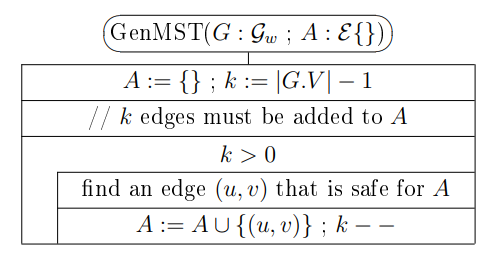
\includegraphics[width=0.65\linewidth]{GenMST}
\end{figure}

\pagebreak

\subsubsection{Vágás (nem tűnik fontosnak)}

\begin{outline}
	\1 $G=(V,E)$ gráf, $\{\} \subset S \subset V$
	\1 Vágás G-n: $(S, V \setminus S)$
	\1 $(u,v) \in E$ él keresztezi a $(S, V \setminus S)$ vágást, ha $u \in S = v \in V \setminus S$
		\2 azaz ha $(u \in S \wedge v \in V \setminus S) \lor (u \in V \setminus S \wedge v \in S)$
	\1 $(u,v) \in E$ könnyű él egy vágásban, ha
		\2 $(u,v)$ keresztezi a vágást
		\2 és $\forall(p,q)$ vágást keresztező élre $w(u,v) \le w(p,q)$
	\1 $A \subseteq E$ élhalmaz elkerüli a vágást, ha $A$ egyetlen éle sem keresztezi azt
\end{outline}

\subsubsection{Tétel biztongságos élre (nem tűnik fontosnak)}

\begin{outline}
	\1 Legyen $g=(V,E)$ irányítatlan, összefüggő, élsúlyozott gráf
	\1 $A$ részhalmaza G valamelyik minimális feszítőfájának élhalmazának
	\1 $(S,V \setminus S)$ vágás elkerüli az $A$ élhalmazt
	\1 $(u,v) \in E$ könnyű él a $(S,V \setminus S)$ vágásban
	\1 Ekkor $(u,v)$ biztonságos él; hozzávehető $A$-hoz
	\1 Bizonyítás: nem nagyon értem, nem tűnik fontosnak, de jegyzetben
\end{outline}

\pagebreak

\subsection{Kruskal algoritmusa}

\begin{outline}
	\1 Legyen $G=(V,E)$ összefüggő, irányítatlan, élsúlyozott gráf
	\1 Invariáns: $(V,A)$ a $G$ egy feszítő erdeje és $A$ részhalmaza $G$ egy MST-jének élhalmazának
	\1 Kezdetben $A=\{\}$. Az éleket súlyuk szerint növekvő sorrendben dolgozzuk fel. Minden új éllel két fát kötünk össze, így a fák száma mindig csökken. Amennyiben egy él nem volt biztonságos, eldobjuk.
\end{outline}

\begin{figure}[h!]
	\centering
	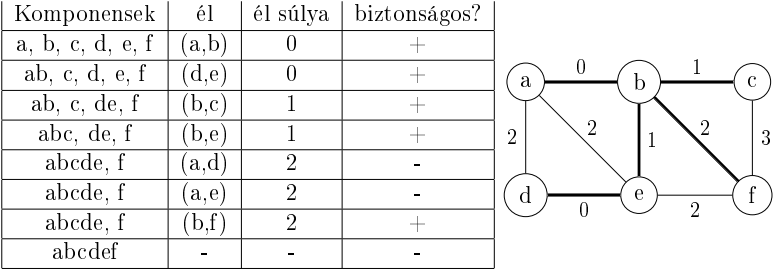
\includegraphics[width=0.9\linewidth]{kruskal-példa}
\end{figure}

\begin{figure}[h!]
	\centering
	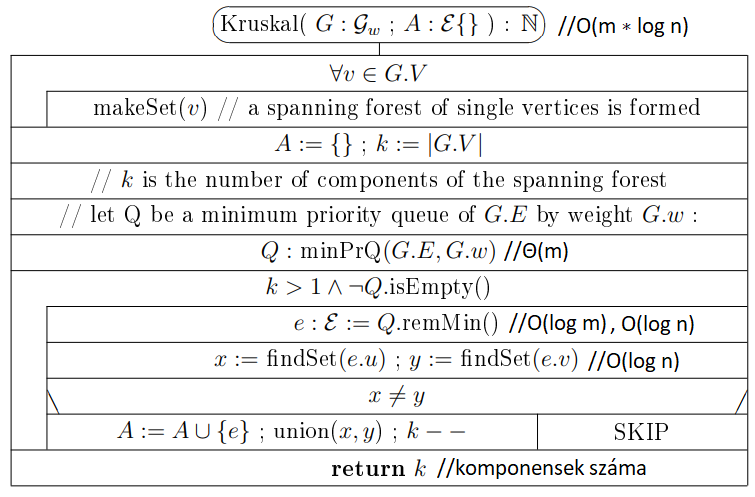
\includegraphics[width=0.9\linewidth]{kruskal}
\end{figure}

\pagebreak

\begin{figure}[h!]
	\centering
	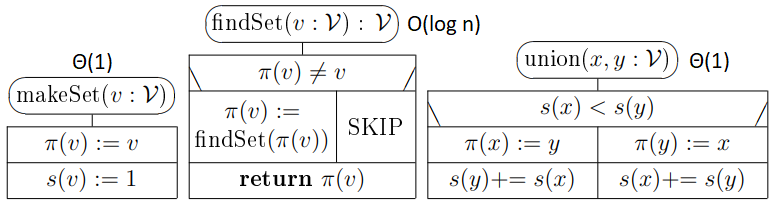
\includegraphics[width=0.9\linewidth]{kruskal-halmaz}
\end{figure}

\begin{outline}
	\1 Az irányítatlan feszítőerdő mellett egy irányított erdőt is kezelünk. Ez az irányított erdő a "gyökere felé mutat".
	\1 $\pi$ címke: szülő csúcsot tárolja, gyökérre viszont $\pi(r)=r$
	\1 $s(r)$ az $r$ gyökérhez tartozó fa mérete
	\1 $union$ mindig a kisebbet fűzi be a nagyobb-egyenlő gyökerébe közvetlenül. Így sosem lesz a fák magassága nagyobb, mint méretük $\log_2$. Ezért lesz a $findSet$ hatékony.
\end{outline}

\pagebreak

\subsection{Prim algoritmusa}

\begin{outline}
	\1 Legyen $G=(V,E)$ összefüggő, irányítatlan, élsúlyozott gráf
	\1 Invariáns: $T=(N,A)$ mindig $G$ egy MST-jének része
	\1 $A$-hoz mindig olyan biztonságos élet adunk hozzá, amelyik él egy $A$-beli és $A$-n kívüli csúcsot köt össze.
	\1 Kezdetben tetszőleges csúcsból indulunk. ($N=\{r\}; \; A=\{\}$)
	\1 Minden $V \setminus N$ csúcshoz tartozik $c$ és $p$ címke, ha van él köztük és a $N$ egyik csúcsa között (azaz a $(N,V \setminus N)$ vágásban)
		\2 $p(u)$: egy vágásban lévő él másik csúcsa; az él: $(p(u),u)$
		\2 $c(u)$: az él súlya; $c(u)=w(p(u),u)$
		\2 mindez úgy, hogy $\forall (x,u)$ vágásbeli élre $w(x,u) \ge w(p(u),u)$
	\1 Ha nincs él $u$ és $N$ egy csúcsa között sem: $p(u)=\emptyset$ és $c(u)=\infty$
	\1 $A$-hoz mindig a $c(u)$ szerint legkisebb élet adjuk hozzá.
		\2 Egy min prioritásos sorban tároljuk az $u$ csúcsokat.
		\2 Egy ilyen hozzáadáskor frissíteni kell a $c(v)$ értékeket minden olyan $v$-re, amelyik szomszédja $u$-nak.
	\1 A végső fa élei $(p(x),x)$, ahol $x \in V \setminus \{r\}$ (csúcshalmaza pedig $V$)
\end{outline}

\pagebreak

\begin{figure}[h!]
	\centering
	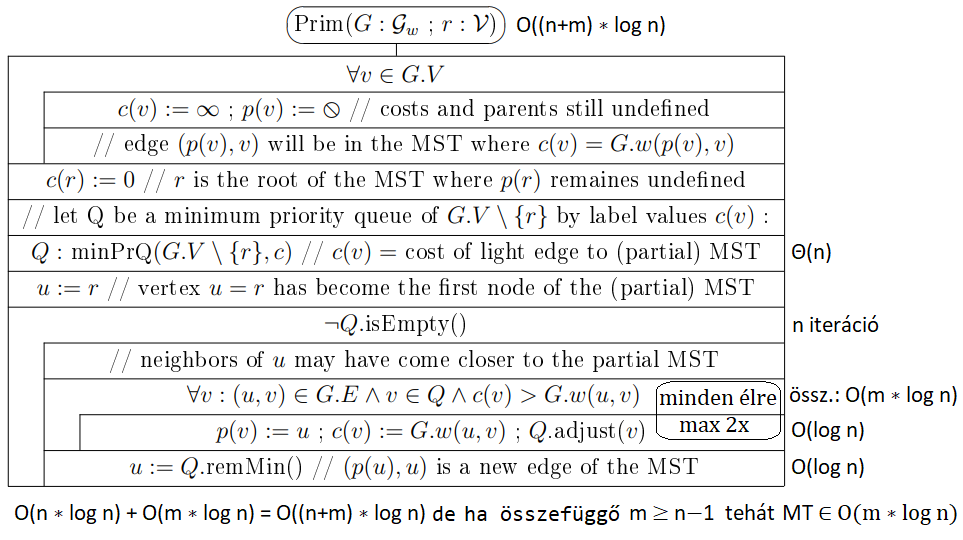
\includegraphics[width=1\linewidth]{prim}
\end{figure}

\begin{figure}[h!]
	\centering
	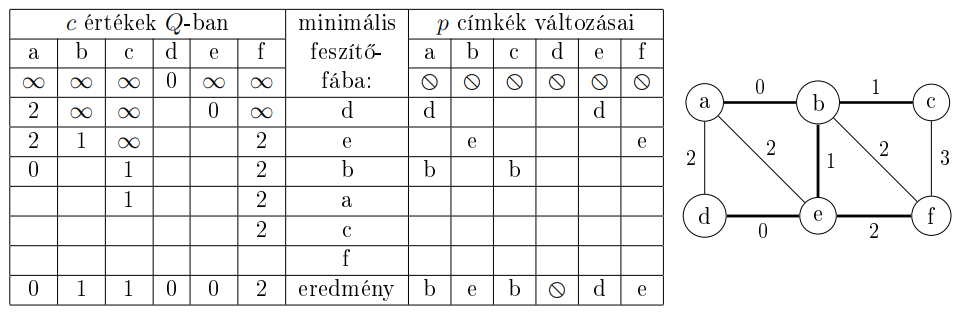
\includegraphics[width=1\linewidth]{prim-példa}
\end{figure}

\pagebreak

\section{Legrövidebb utak egy forrásból}

\begin{outline}
	\1 Adott $s$ csúcsból minden $s$-ből elérhető csúcsba legrövidebb utat keresünk.
	\1 Értelmezzük az irányítatlan gráfot olyan irányított gráfként,\\
	ahol $(u,v) \in E \implies (v,u) \in E \wedge w(u,v) = w(v,u)$
	\1 Pontosan akkor oldható meg, ha nem létezik $s$-ből elérhető negatív kör
		\2 Negatív kör: olyan kör, amelynek összsúlya negatív
		\2 Irányítatlan gráfok esetén akkor is lesz ilyen "kör", ha van negatív súlyú él.
	\1 Ha megoldható, mindegyik $v \in V \setminus \{s\}$-re két lehetőség van:
		\2 Létezik út $s$-ből $v$-be:
			\3 $d(v)$ az optimális út hossza
			\3 $\pi(v)$ az optimális úton $v$-t közvetlenül megelőző csúcs
		\2 Nem létezik út $s$-ből $v$-be: $d(v)=\infty$ és $\pi(v)=\emptyset$
		\2 $s$ csúcsra: $d(s)=0$ és $\pi(s)=\emptyset$
	\1 Az algoritmusok az optimális utat folyamatosan közelítik, $d(v)=\infty$ és $\pi(v)=\emptyset$-ből indulva. Jelölje $s \leadsto v$ azt a kiszámolt utat, ami az eddigi legjobb; ekkor $d(v)\in \mathbb{R}$ és $v \ne s$ esetén $\pi(v) \ne \emptyset$. Gráf éleit folyamatosan vizsgáljuk és ha pl. $(u,v)$-t nézzük éppen és $s\leadsto u \to v$ rövidebb,
	mint $s \leadsto v$, akkor frissítjük: közelítjük (relaxation).
	\1 Az algoritmusok közös vonása, hogy egy feldolgozandó csúcsok halmazából minden lépésben kivesznek egy csúcsot és az összes kimenő élre elvégzik a közelítést. A közelítéseket a csúcs kiterjesztésének nevezzük. A csúcs kivételét és a kiterjesztést együtt pedig a csúcs feldolgozásának.
\end{outline}

\pagebreak

\subsection{Dijkstra algoritmusa}

\begin{outline}
	\1 Előfeltétel: mindegyik él súlya nemnegatív
	\1 Nagyon hasonlít Prim algoritmusára, mohó
		\2 $MT \in O((n+m)*\lg n)$ (magyarázat: Prim algoritmusa)
		\2 $mT \in \Theta(n)$ (ha $s$-nek nincs rákövetkezője)
\end{outline}

\begin{figure}[h!]
	\centering
	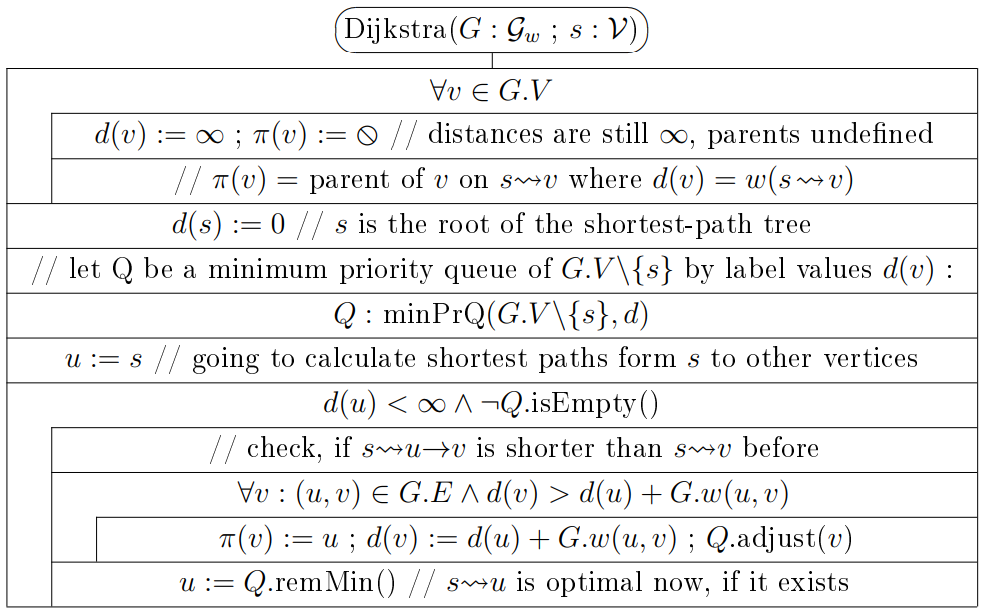
\includegraphics[width=0.9\linewidth]{dijkstra}
\end{figure}

\begin{figure}[h!]
	\centering
	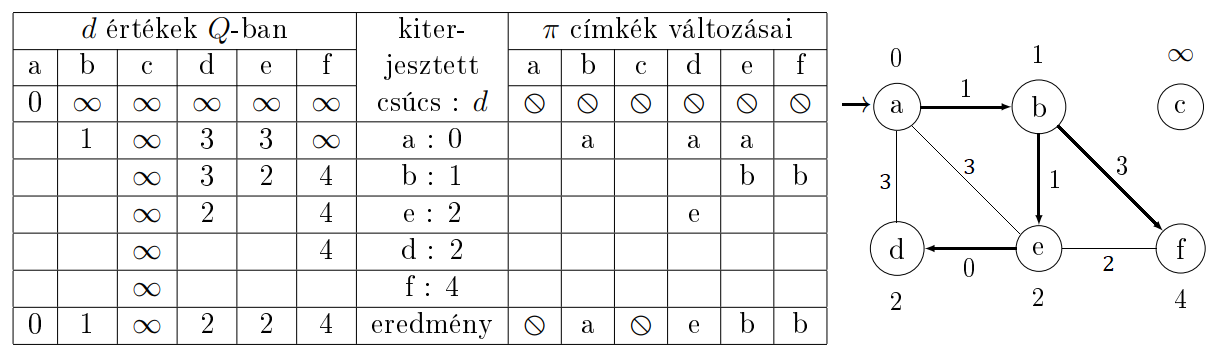
\includegraphics[width=1\linewidth]{dijkstra-példa}
\end{figure}

\begin{outline}
	\1 $u:=Q.remMin()$-nél $s \leadsto u$ optimális ha $d(u) \ne \infty$. Bizonyítás indirekt módon, jegyzetben.
	\1 Ha $u:=Q.remMin()$-nél $d(u) = \infty$ akkor $Q$ egy eleme sem érhető el $s$-ből.
	% Bizonyítás: mindig a minimális súlyút vesszük ki a sorból, tehát ha $d(u)=\infty$ akkor egy csúcs $d$ értéke sem fog csökkenni. Tehát ha $d(u)$ volt a legkisebb, akkor már minden maradék $Q$-beli csúcs elérhetetlen.
\end{outline}

\pagebreak

\subsection{DAGshP (DAG shortest Paths)}

\begin{outline}
	\1 Előfeltétel: irányított a gráf és nincs benne irányított kör
	\1 Az algoritmus ellenőrzi az előfeltételét:
		\2 nincs irányított kör: $\emptyset$-tel tér vissza
		\2 különben a kör egy csúcsával tér vissza, ami a $\pi$ címkék mentén fordított irányban bejárható
	\1 $MT \in \Theta(n+m)$ és $mT \in \Theta(n)$
	\1 A $topologicalSort$ csak az $s$-ből elérhető részgráfot teszi be $S$-be, a megfelelő sorrendben.
	\1 A $time$ változó globális, de csak szemléltetésre van, elhagyható.
\end{outline}

\begin{figure}[h!]
	\centering
	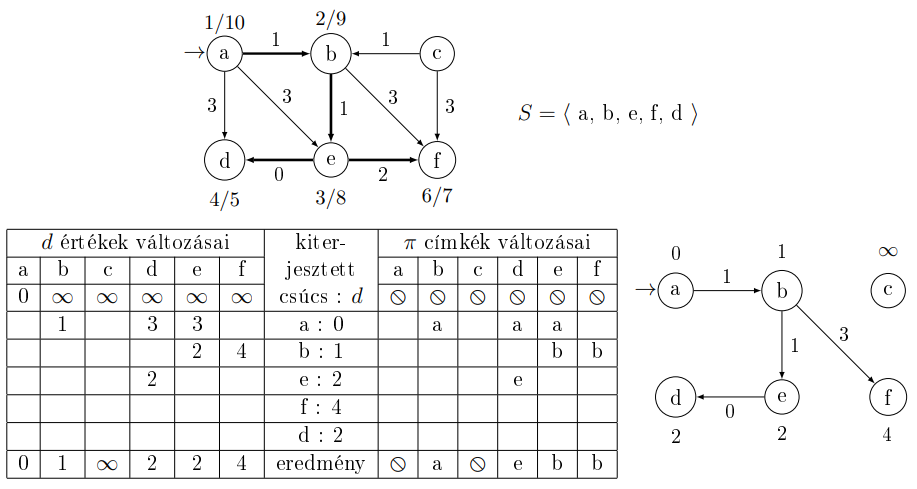
\includegraphics[width=1\linewidth]{DAGshP-példa}
\end{figure}

\pagebreak

\begin{figure}[h!]
	\centering
	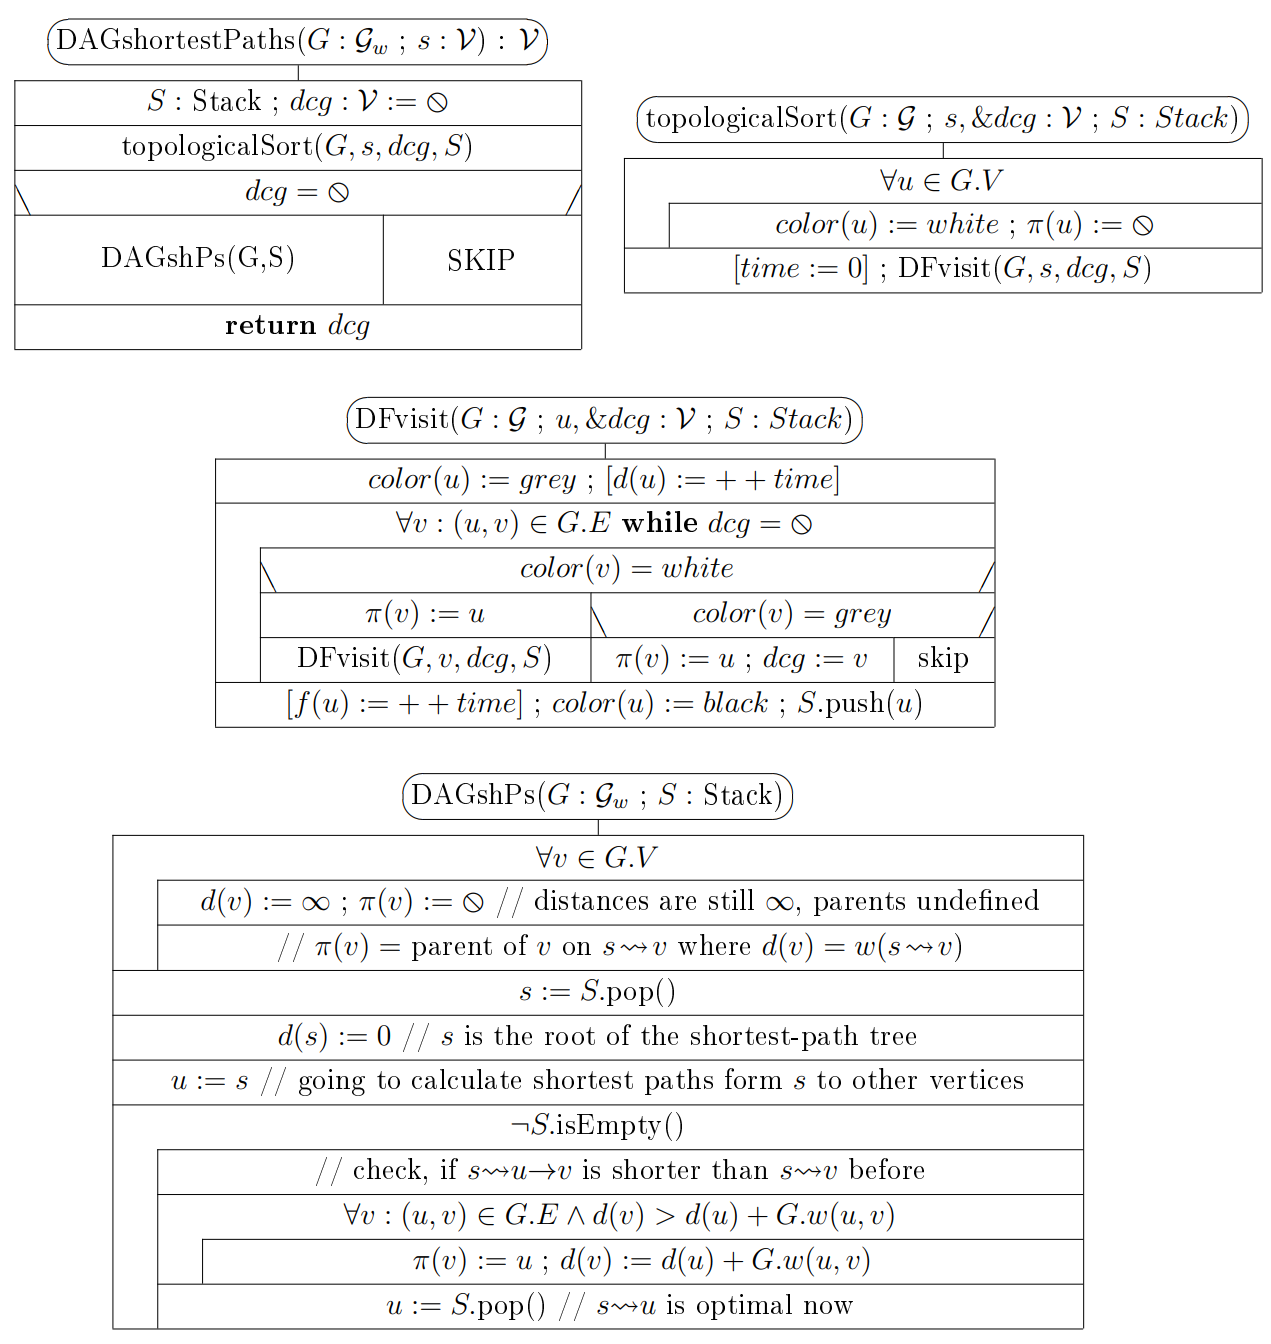
\includegraphics[width=1\linewidth]{DAGshP}
\end{figure}

\pagebreak

\subsection{Sor-alapú Bellman-Ford algoritmus (QBF)}

\begin{outline}
	\1 Nem mohó
	\1 Előfeltétel: nincs $s$-ből elérhető negatív kör.
	\1 Előfeltétel ellenőrzése algoritmusban:
		\2 $e(v)$ címke: $s \leadsto v$ út élszáma (NEM súlya!)
		\2 nincs negatív kör: $e(v) < n$ és $\emptyset$ a visszatérési érték
		\2 $e(v) \ge n \implies$ $v$ része egy negatív körnek, vagy $\pi(v)$-n keresztül negatív körbe érkezünk (max $n$ lépésben megoldható), a kör egyik csúcsa a visszatérési érték
	\1 $MT = O(n*m)$
		\2 gyakorlatban átlagosan $\Theta(n)$, ha ritka a gráf ($m \in O(n)$)
	\1 Új címke: $inQ$ (benne van-e a sorban, bit tömbbel megvalósítható)
\end{outline}

\begin{figure}[h!]
	\centering
	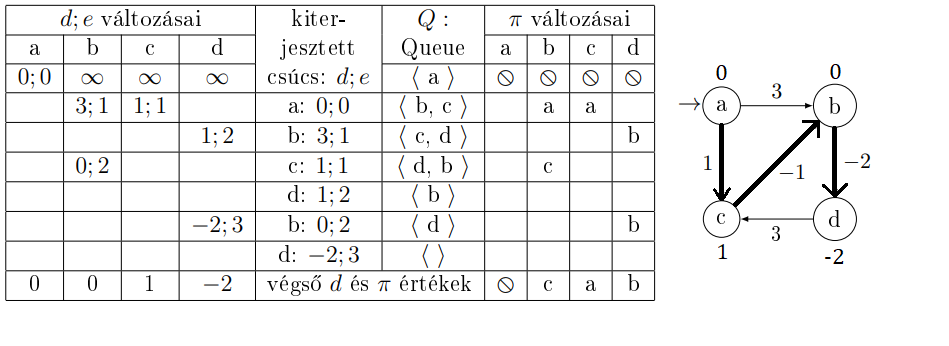
\includegraphics[width=1\linewidth]{QBF-példa-jó}
\end{figure}

\begin{figure}[h!]
	\centering
	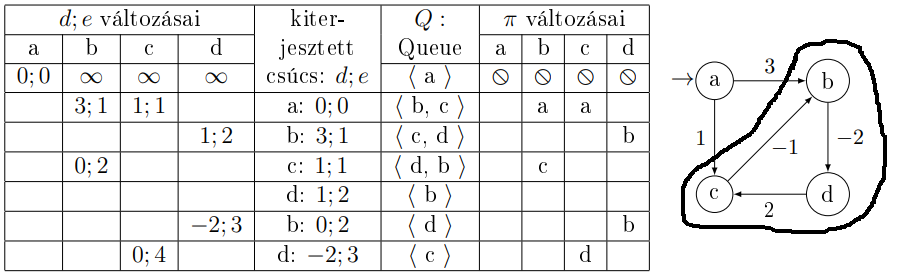
\includegraphics[width=1\linewidth]{QBF-példa-kör}
\end{figure}

\pagebreak

\begin{figure}[h!]
	\centering
	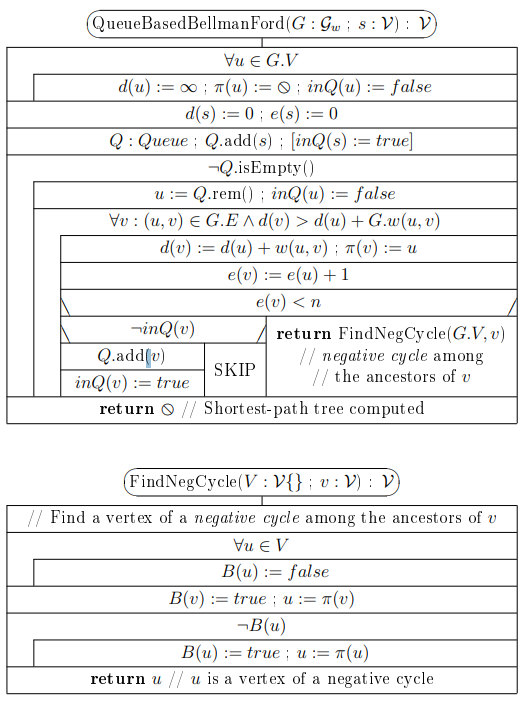
\includegraphics[width=0.7\linewidth]{QBF}
\end{figure}

\begin{outline}
	\1 Menet:
		\2 0.: $s$ feldolgozása
		\2 $(i+1)$.: $i$. menet lévén sorban lévő csúcsok feldolgozása
	\1 Ha $s$-ből nem érhető el negatív kör:
		\2 Ha $s \leadsto u$ optimális út $k$ élből áll, akkor a k. menet elején már megtalálta az algoritmus.
		\2 Minden optimális út max $n-1$ hosszú $\implies$ n-1. menet végére kiürül a sor. Innen jön $MT \in O(n*m)$.
\end{outline}

\pagebreak

\section{Legrövidebb utak minden csúcspárra}

\subsection{Floyd-Warshall (FW) algoritmus}

\begin{outline}
	\1 Legyen $\mathbb{R}_\infty = \mathbb{R} \cup \{\infty\}$, ahol $\infty$ jelentése: nincs él/út
	\1 Mátrixok kiolvasása, $A[i,j]$ jelentése: $i$-ből (sor) $j$-be (oszlop) valami
	\1 Bemenet: élsúlyozott gráf egy $A/1: \mathbb{R}_\infty[n,n]$ csúcsmátrixként
	\1 Kimenet:
		\2 Utak hossza: $D/1: \mathbb{R}_\infty[n,n]$
		\2 Útban a csúcs megelőzője: $\pi/1: \mathbb{N}[n,n]$
			\3 Ha nincs út, vagy $i=j$ akkor: $\pi[i,j]=\emptyset$
	\1 Előfeltétel (ellenőrzi magától): gráfban nincs negatív kör
		\2 Visszatér egy negatív körbeli csúccsal, ha van ilyen.
\end{outline}

\begin{figure}[h!]
	\centering
	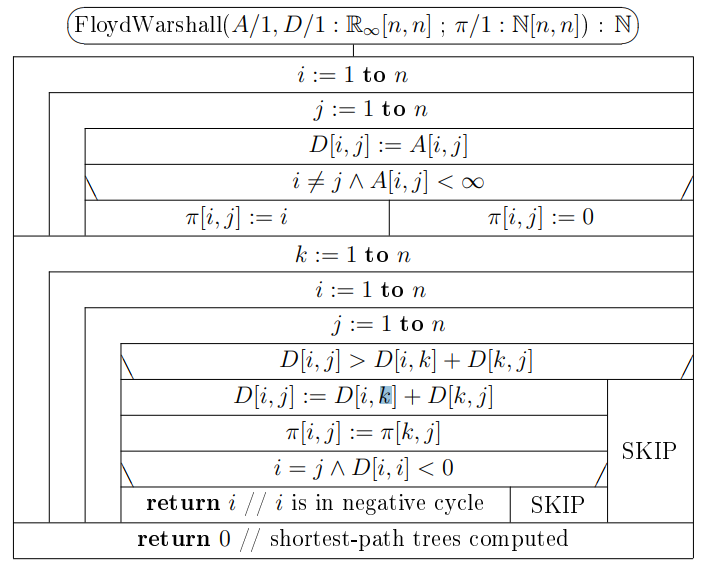
\includegraphics[width=0.7\linewidth]{FloydWarshall}
\end{figure}

\begin{outline}
	\1 Műveletigény: $MT(n) \in \Theta(n^3)$
		\2 Ha van negatív kör, akkor $mT(n) \in \Theta(n^2)$ \; (egyébként $\Theta(n^3)$)
\pagebreak
	\1 Megoldás módszere: dinamikus programozás
		\2 két csúcs ($i$ és $j$) között az első $k$ csúcs felhasználásával keresünk utat
		($i > k$ és $j > k$ megengedett)
		\2 $\exists i \leadsto^0_{opt} j$ ha $(i,j) \in G.E$ \;\; (ekkor az út: $<i,j>$)
		\2 $\forall k \in 1..n: i \leadsto^{k}_{opt} j$ vagy $i \leadsto^{k-1}_{opt} j$
		vagy $i \leadsto^{k-1}_{opt} k \leadsto^{k-1}_{opt} j$
		\2 Ha az $i$-ből $i$-be vezető optimális út súlya negatív, akkor (és csak akkor) van negatív kör és ekkor $i$ a negatív kör része.
\end{outline}

\subsection{Visszavezetés az "utak egy forrásból" feladatra}

\begin{outline}
	\1 Floyd-Warshall algoritmus $D$ és $\pi$ mátrixának $i$-edik sora a "legrövidebb utak egy forrásból" feladat megoldása $s=i$ esetre, valamint fordítva.
	\1 Fontos: a DAG és Dijkstra algoritmusok előfeltétele szigorúbb.
	\1 A DAG algoritmus $n$-szer meghívva: $MT \in \Theta(n*(n+m))$
		\2 Ritka gráfon aszimptotikusan jobb: $\Theta(n^2)$
		\2 Sűrű gráfon egyenlő ($\Theta(n^3)$), gyakorlatban lassabb
	\1 Dijkstra algoritmust $n$-szer meghívva: $MT \in \Theta(n*(n+m)*\log n)$
		\2 Ritka gráf: $\Theta(n^2*\log n)$ (tehát jobb)
		\2 Sűrű gráf: $\Theta(n^3*\log n)$ (tehát rosszabb)
	\1 QBF algoritmust $n$-szer meghívva: $MT \in \Theta(n^2*m)$
		\2 Ez soha nem jobb, legkedvezőbb esetben aszomptotikusan azonos
\end{outline}

\pagebreak

\section{Gráf tranzitív lezártja (Transitive Closure)}

\begin{outline}
	\1 Gráfban honnét hova lehet eljutni (konkrét út és súly lényegtelen)
	\1 $G=(V,E)$ tranzitív lezártja a $T \subseteq V \times V$ reláció, ahol:\\
	$(u,v) \in T \Leftrightarrow$ $G$-ben az $u$ csúcsból elérhető a $v$ csúcs
\end{outline}

\subsection{Egyszerű algoritmus}

\begin{outline}
	\1 Bemenet: gráf egy $A/1:\mathbb{B}[n,n]$ csúcsmátrixként
	\1 Kimenet: $T/1:\mathbb{B}[n,n]$ ahol $T[i,j]=$ van út $i$-ből (sor) $j$-be (oszlop)
	\1 Megoldási módszer: dinamikus programozás, $mT=MT \in \Theta(n^3)$
		\2 $T^{(0)}_{i,j}=\exists i \leadsto j$ az első $k$ csúcsot használva csak ($i,j>k$ szabad)
		\2 $T^{(0)}_{i,j}=A[i,j] \lor (i=j)$
		\2 $T^{k}_{i,j}=T^{k-1}_{i,j} \lor (T^{k-1}_{i,k} \wedge T^{k-1}_{k,j})$
	\1 Floyd-Warshall kimenetből megadható: $T[i,j] = D[i,j] < \infty$\\
	(de FW-nek van előfeltétele és gyakorlatban nem annyira hatékony)
\end{outline}

\begin{figure}[h!]
	\centering
	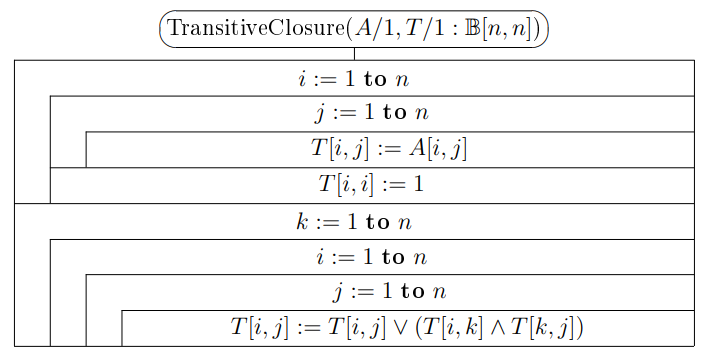
\includegraphics[width=0.7\linewidth]{TransitiveClosure}
\end{figure}

\subsection{Visszavezetés szélességi keresésre}

\begin{outline}
	\1 A kimeneti mátrix $i$-edik sora a BFS $s=i$ kimenetéből kiszámolható:\\
	$\forall j: T[i,j] \Leftrightarrow \pi(j) \ne \emptyset$ \;\;
	(vagy $color(j) \ne white$ vagy $d(j) \ne \infty$)
	\1 BFS $n$-szeri lefuttatása: $MT \in \Theta(n*(n+m))$
		\2 Ritka gráfon aszimptotikusan jobb: $\Theta(n^2)$
		\2 Sűrű gráfon egyenlő ($\Theta(n^3)$), gyakorlatban lassabb
\end{outline}

\end{document}
